\chapter{More on Vector Geometry}

Vectors are a great tool to describe geometry. In this chapter we are going to exploit the knowledge learnt in the previous chapter to solve geometric problems.
\section{Lines and Planes}
Lines and planes are geometric objects of importance in 2D and 3D spaces and they are the first topics to be discussed. They can be expressed in terms of
(a) Equations, and (b) Vectors. We will start from talking lines which is easier.\\
\\
Since a line is a 1D object, the vector form of a line can be expressed mainly by a vector along its direction, times an arbitrary parameter which controls its length by extension or contraction, together with another arbitrary, fixed vector that represents its initial position.
\begin{center}
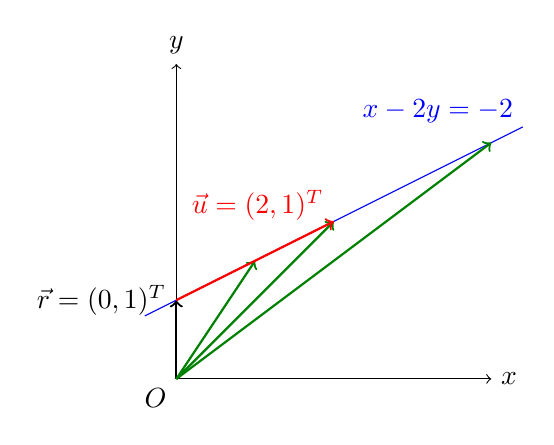
\begin{tikzpicture}
\draw[->] (0,0)--(4,0) node[right]{$x$};
\draw[->] (0,0)--(0,4) node[above]{$y$};
\draw[thick, ->] (0,0)--(0,1) node[left]{$\vec{r} = (0,1)^T$};
\draw[blue] (-0.4, 0.8)--(4.4, 3.2) node[left, shift={(0mm, 2mm)}]{$x - 2y = -2$};
\draw[Green, thick, ->] (0,0)--(2,2);
\draw[Green, thick, ->] (0,0)--(4,3);
\draw[Green, thick, ->] (0,0)--(1,1.5);
\draw[red, thick, ->] (0,1)--(2,2) node[left, shift={(0mm, 2mm)}]{$\vec{u} = (2,1)^T$};
\node[below left]{$O$}; 
\end{tikzpicture}\\
$\textcolor{Green}{\overrightarrow{OP}} = \vec{r} + \textcolor{blue}{t} \textcolor{red}{\vec{u}} = (0,1)^T + \textcolor{blue}{t} \textcolor{red}{(2,1)^T}$, the green arrow is controlled by $\textcolor{blue}{t}$ like a slider, the above graph shows the cases for $\textcolor{blue}{t} = 0.5, 1, 2$.
\end{center}
Short Exercise: Choose any value of $t$ and substitute it into the expression of $\overrightarrow{OP}$ to see if the $x$ and $y$-components satisfy the equation. Also, try to increase/decrease the value of $t$ to observe how the vector traces out a line.

\subsection{Translating Equation Form to Vector Form}
General form of equation of a line on x-y plane is $ax + by = h$, resembling a linear system of one equation with two unknowns. From Section \ref{subsection:SolLinSysGauss}, it can be observed that it has infinitely many solutions and possesses a free variable. Let $y = t$, then rearranging the equation we have $x = (h - bt)/a$ where $t$ is any scalar. Denote the origin as $O$ and any point on the line as $P$, then the vector from the origin to the line is
\begin{align*}
\overrightarrow{OP} =
\begin{bmatrix}
x \\
y
\end{bmatrix}
=
\begin{bmatrix}
\frac{h}{a} - \frac{b}{a}t\\
t
\end{bmatrix}
= 
\begin{bmatrix}
\frac{h}{a}\\
0
\end{bmatrix}
+ t
\begin{bmatrix}
-\frac{b}{a}\\
1
\end{bmatrix}
\end{align*}
This is the vector form of the line. The ideas behind can be borrowed from Example \ref{MulSol}, with $(h/a, 0)^T$ being the particular solution/initial position, and $(-b/a, 1)^T$ being the general solution/direction. For example, if we have $3x - 2y = 5$, then by the same method, we get
\begin{align*}
\begin{bmatrix}
x \\
y
\end{bmatrix}
=
\begin{bmatrix}
\frac{5}{3} + \frac{2}{3}t\\
t
\end{bmatrix}
= 
\begin{bmatrix}
\frac{5}{3}\\
0
\end{bmatrix}
+ t
\begin{bmatrix}
\frac{2}{3}\\
1
\end{bmatrix}    
\end{align*}
Bear in mind that the direction vector (general solution) can be scaled freely. In addition, any initial position vector (particular solution) can be chosen as long as it links to a point on the line, satisfying the equation. Hence there is no unique vector form for a line. For instance,
\begin{align*}
\begin{bmatrix}
1\\
3
\end{bmatrix}
+ t_1
\begin{bmatrix}
2 \\
4
\end{bmatrix}     
\end{align*}
is equivalent to
\begin{align*}
\begin{bmatrix}
-1\\
-1
\end{bmatrix}
+ t_2
\begin{bmatrix}
1 \\
2
\end{bmatrix}     
\end{align*}
for the line equation $2x - y = -1$.\\
Short Exercise: Verify the equivalence by choosing a value for $t_1$ and finding the corresponding $t_2$ so that the vector points to the same position.

\subsection{Recovering Equation Form from Vector Form} On the other hand, inferring line equation from the vector form is not straight-forward at first sight. Since the vector form of a line always contains an arbitrary parameter, which is absent in the equation form, the motivation is to remove the parameter through some manipulation.\\
\\
Remember that from Properties \ref{dotorth} the dot product between orthogonal (perpendicular) vectors returns zero. This means that by carrying out dot product with the vector orthogonal to the direction vector, namely the normal vector, on both sides of the vector form will eliminate the parameter and recover the line equation. For example, given that
\begin{align*}
\begin{bmatrix}
x\\
y
\end{bmatrix}
=
\begin{bmatrix}
1\\
3
\end{bmatrix}
+ t
\begin{bmatrix}
1 \\
4
\end{bmatrix} 
\end{align*}
We know that $(4, -1)^T$ is a vector orthogonal to the direction. So, by taking dot product with $(4, -1)^T$ on both sides, we have
\begin{align*}
\begin{bmatrix}
x\\
y
\end{bmatrix}
\cdot
\begin{bmatrix}
4\\
-1
\end{bmatrix}
&=
\begin{bmatrix}
1\\
3
\end{bmatrix}
\cdot
\begin{bmatrix}
4\\
-1
\end{bmatrix}
+ t
\begin{bmatrix}
1 \\
4
\end{bmatrix} 
\cdot
\begin{bmatrix}
4\\
-1
\end{bmatrix}\\
4x - y &= 1 + (0)t = 1
\end{align*}
Notice that the coefficients are the same as the components of the normal vector.\\
Short Exercise: Verify that $(a, b)$ is always orthogonal to $(b, -a)$, and vice versa.

\subsection{Generalizing to Higher Dimension}
Similar concepts can be applied on the equation and vector form for planes. General form of equation of a plane in 3D space is $ax + by + cz = h$, which is a linear system of one equation with three unknowns, implying two free variables and two direction vectors for such plane. By doing Gaussian Elimination, we obtain the vector form of the plane. \\
\\
Cross product of any two non-parallel vectors on the plane will give the third vector normal to the plane, then we can take the dot product with this new vector to convert the vector form back into a plane equation. Again, the coefficients of the plane equation match the components of the normal vector, differed at most by a factor.
\begin{center}
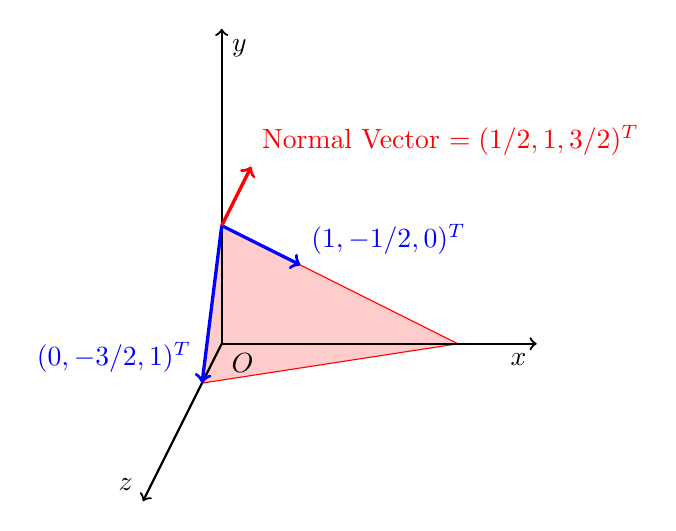
\begin{tikzpicture}[z={(-0.25,-0.5)}]
\filldraw[draw=red, fill=red!20]
(3,0,0) -- (0,3/2,0) -- (0,0,1) -- cycle;
\node[below right]{$O$}; 
\draw[thick,->] (0,0,0) -- (4,0,0) node[anchor=north east]{$x$};
\draw[thick,->] (0,0,0) -- (0,4,0) node[anchor=north west]{$y$};
\draw[thick,->] (0,0,0) -- (0,0,4) node[anchor=south east]{$z$};
\draw[very thick,->,blue] (0,3/2,0) -- (1,1,0) node[above right]{$(1, -1/2, 0)^T$};
\draw[very thick,->,blue] (0,3/2,0) -- (0,0,1) node[above left]{$(0, -3/2, 1)^T$};
\draw[very thick,->,red] (0,3/2,0) -- (3/2,9/2,9/2) node[above right]{Normal Vector $= (1/2, 1, 3/2)^T$};
\end{tikzpicture} \\
The plane represented by the equation $x + 2y + 3z = 3$. Notice that the normal vector can be found via computing $(0, -3/2, 1)^T \times (1, -1/2, 0)^T = (1/2, 1, 3/2)^T$. The normal vector is magnified for the purpose of illustration.
\end{center}

\begin{exmp}
For the equation $2x+3y+z = 4$, we can let $y=s$, $z=t$, then
\begin{align*}
\begin{bmatrix}
x \\
y \\
z
\end{bmatrix}
=
\begin{bmatrix}
(4-3s-t)/2 \\
s \\
t
\end{bmatrix}
=
\begin{bmatrix}
2 \\
0 \\
0
\end{bmatrix}
+ s
\begin{bmatrix}
-3/2 \\
1 \\
0
\end{bmatrix}
+ t
\begin{bmatrix}
-1/2 \\
0 \\
1
\end{bmatrix}
\end{align*}
where $-\infty < s < \infty$, $-\infty < t < \infty$ are some scalars. To recover the original equation, we can find the normal vector by doing cross product on the two vectors representing the general solutions.
\begin{align*}
\begin{bmatrix}
-3/2 \\
1 \\
0
\end{bmatrix}
\times
\begin{bmatrix}
-1/2 \\
0 \\
1
\end{bmatrix}
=
\begin{vmatrix}
\hat{i} & \hat{j} & \hat{k} \\
-3/2 & 1 & 0 \\
-1/2 & 0 & 1
\end{vmatrix}
= \hat{i} + \frac{3}{2}\hat{j} + \frac{1}{2}\hat{k}
\end{align*}
The next step is to take the dot product with the normal vector obtained above.
\begin{align*}
\begin{bmatrix}
x \\
y \\
z
\end{bmatrix}
&=
\begin{bmatrix}
2 \\
0 \\
0
\end{bmatrix}
+ s
\begin{bmatrix}
-3/2 \\
1 \\
0
\end{bmatrix}
+ t
\begin{bmatrix}
-1/2 \\
0 \\
1
\end{bmatrix} \\
\begin{bmatrix}
x \\
y \\
z
\end{bmatrix}
\cdot
\begin{bmatrix}
1 \\
3/2 \\
1/2
\end{bmatrix}
&=
\begin{bmatrix}
2 \\
0 \\
0
\end{bmatrix}
\cdot
\begin{bmatrix}
1 \\
3/2 \\
1/2
\end{bmatrix}
+ s
\begin{bmatrix}
-3/2 \\
1 \\
0
\end{bmatrix}
\cdot
\begin{bmatrix}
1 \\
3/2 \\
1/2
\end{bmatrix}
+ t
\begin{bmatrix}
-1/2 \\
0 \\
1
\end{bmatrix}
\cdot
\begin{bmatrix}
1 \\
3/2 \\
1/2
\end{bmatrix} \\
x + \frac{3}{2}y + \frac{1}{2}z &= 2 + (0)s + (0)t = 2
\end{align*}
\end{exmp}
The correspondence coefficients of a linear equation and its normal vector is not a coincidence. In fact, even for higher dimensional cases, where there is no simple geometric interpretation, we still have the following results.
\begin{thm}
\label{normalvec}
For an equation in the form of $a_1x_1 + a_2x_2 + a_3x_3 + \cdots + a_nx_n = h$, it has a normal vector of $(a_1, a_2, a_3, \cdots, a_n)^T$.
\end{thm}
The procedures carried in the last example can be similarly applied to higher dimensional circumstances.

\section{More on Geometric Applications of Dot Product}
\subsection{Projection}
The projection of a vector onto another vector can be derived from trigonometry and dot product. 
\begin{center}
\begin{tikzpicture}[scale=1.3]
\coordinate (0) at (0,0);
\draw[->](0)--(4,1) node[right](vecu){$\vec{u}$};
\draw[->](0)--(1,2) node[above](vecv){$\vec{v}$};
\draw[dotted] (1,2)--(24/17, 6/17);
\draw[red] (24/17+0.2, 6/17+0.05)--(24/17+0.15, 6/17+0.25)--(24/17-0.05, 6/17+0.2);
\pic[draw, ->, "$\theta$",angle eccentricity=1.5] {angle = vecu--0--vecv};
\draw[blue, very thick] (0,0)--(24/17, 6/17) node[below, shift={(0mm, -2mm)}]{$\norm{\vec{u}}\cos\theta$};
\end{tikzpicture}
\end{center}
By rearranging the relation stated in Properties \ref{dotgeo}, we have the magnitude of the projection of $\vec{u}$ onto $\vec{v}$ as
\begin{proper}
\label{proj}
Denote the projection of $\vec{u}$ onto $\vec{v}$ by $\text{proj}_v \vec{u}$, where $\vec{u}$ and $\vec{v}$ are both $m$-dimensional, then
\begin{align*}
\norm{\text{proj}_v \vec{u}} = \norm{\vec{u}} \cos\theta = \frac{\vec{u} \cdot \vec{v}}{\norm{\vec{v}}}    
\end{align*}
If we want to have the projection in the form of a vector, then we can utilize the unit vector along $\vec{v}$.
\begin{align*}
\text{proj}_v \vec{u} = \frac{\vec{u} \cdot \vec{v}}{\norm{\vec{v}}} \hat{v} = \frac{\vec{u} \cdot \vec{v}}{\norm{\vec{v}}^2} \vec{v} 
\end{align*}
where we have used Definition \ref{unitvec} for the second equation.
\end{proper}

\begin{exmp}
Find the projection of $\vec{u} = 2\hat{i} - 3\hat{j} + \hat{k}$ onto $\vec{v} = 4\hat{i} + \hat{j} - 3\hat{k}$ using Properties \ref{proj}.
\begin{align*}
\text{proj}_v \vec{u} &= \frac{\vec{u} \cdot \vec{v}}{\norm{\vec{v}}^2} \vec{v} \\
&= \frac{(2)(4)+(-3)(1)+(1)(-3)}{(4)^2+(1)^2+(-3)^2} (4\hat{i} + \hat{j} - 3\hat{k}) \\
&= \frac{1}{13} (4\hat{i} + \hat{j} - 3\hat{k}) = \frac{4}{13}\hat{i} + \frac{1}{13}\hat{j} - \frac{3}{13}\hat{k}
\end{align*}
The length of the projection is $\norm{\text{proj}_v \vec{u}} = \sqrt{(\frac{4}{13})^2 + (\frac{1}{13})^2 + (-\frac{3}{13})^2} = \frac{\sqrt{26}}{13}$.
\end{exmp}

\subsection{Distance} Distance of a point to a line/plane can be found by the projection of any vector connecting the point to the line/plane onto the normal vector of that line/plane, as shown in the figure below.
\begin{center}
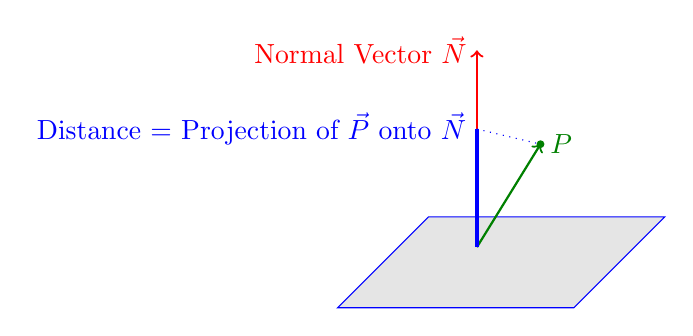
\begin{tikzpicture}
\filldraw[draw=blue, fill=gray!20]
(0,0,0) -- (3,0,0) -- (3,0,3) -- (0,0,3) -- cycle;
\draw[thick,->,red] (1,0,1) -- (1,2.5,1) node[left]{Normal Vector $\vec{N}$};
\coordinate[label = {[Green]right:$P$}] (P) at (2,1.5,1.5);
\node at (P) [circle,fill,inner sep=1pt,Green]{};
\draw[thick,->,Green] (1,0,1) -- (2,1.5,1.5);
\draw[dotted, blue] (1,1.5,1) -- (2,1.5,1.5);
\draw[very thick, blue] (1,0,1) -- (1,1.5,1) node[left]{Distance = Projection of $\vec{P}$ onto $\vec{N}$};
\end{tikzpicture}
\end{center}

\begin{exmp}
Find the distance from the plane $x-2y+3z = 6$ to the point $(3,3,6)^T$.\\
\\
From the equation of the plane, and by Theorem \ref{normalvec}, it can be inferred that the normal vector of the plane is $\hat{i} - 2\hat{j} + 3\hat{k}$. We can select any point on the plane as we wish, let's say $(4,2,2)^T$, and the vector connecting it to the point $(3,3,6)^T$ is simply their difference $-\hat{i} + \hat{j} + 4\hat{k}$. Then the distance is found from the length of the projection of $-\hat{i} + \hat{j} + 4\hat{k}$ onto the normal vector of the plane $\hat{i} - 2\hat{j} + 3\hat{k}$. By Properties \ref{proj}, it is
\begin{align*}
\frac{(-\hat{i} + \hat{j} + 4\hat{k}) \cdot (\hat{i} - 2\hat{j} + 3\hat{k})}{\norm{\hat{i} - 2\hat{j} + 3\hat{k}}} = \frac{(-1)(1)+(1)(-2)+(4)(3)}{\sqrt{(1)^2 + (-2)^2 + (3)^2}} = \frac{9}{\sqrt{14}}
\end{align*}
\end{exmp}
Sometimes the calculation may lead to a negative value for the projection and we may want to take the absolute value.

\section{More on Geometric Applications of Cross Product}
\subsection{Area}
The area of the parallelogram formed by two vectors $\vec{u}$, $\vec{v}$ are simply the absolute value of their cross product.
\begin{center}
\begin{tikzpicture}
\coordinate (0) at (0,0);
\draw[thick, ->] (0)--(4,0) node[right](vecu){$\vec{u}$};
\draw[thick, ->] (0)--(1,3) node[above left](vecv){$\vec{v}$};
\draw[thick, ->, gray] (4,0)--(5,3);
\draw[thick, ->, gray] (1,3)--(5,3);
\draw[dotted, blue] (1,3)--(4,0);
\draw[dotted, gray] (1,3)--(1,0) node[midway, right]{$\norm{\vec{v}}\sin\theta$};
\draw[red] (1+0.15, 0)--(1+0.15, 0+0.15)--(1, 0+0.15);
\pic[draw, ->, "$\theta$",angle eccentricity=1.5] {angle = vecu--0--vecv};
\end{tikzpicture}
\end{center}
\begin{proper}
\label{parallelogram}
Directly by Properties \ref{crossgeo}, the area of the parallelogram formed by two vectors $\vec{u}$, $\vec{v}$ is
\begin{align*}
\norm{\vec{u} \times \vec{v}} = \norm{\vec{u}}\norm{\vec{v}}\sin\theta
\end{align*}
Similarly, the triangle built by $\vec{u}$, $\vec{v}$ is half of the quantity above, as
\begin{align*}
\frac{1}{2}\norm{\vec{u} \times \vec{v}} = \frac{1}{2}\norm{\vec{u}}\norm{\vec{v}}\sin\theta   
\end{align*}
\end{proper}

\begin{exmp}
Find the area of the parallelogram formed by $\vec{u} = (-1, -2, 4)^T$ and $\vec{v} = (3, 0, 1)^T$.\\
\\
The cross product between the given two vectors is
\begin{align*}
\vec{u} \times \vec{v} &=
\begin{vmatrix}
\hat{i} & \hat{j} & \hat{k} \\
-1 & -2 & 4 \\
3 & 0 & 1
\end{vmatrix} \\
&= -2\hat{i} + 13\hat{j} + 6\hat{k}
\end{align*}
Therefore, the required area is
\begin{align*}
\norm{\vec{u} \times \vec{v}} &= \sqrt{(-2)^2 + (13)^2 + (6)^2} \\
&= \sqrt{209}
\end{align*}
\end{exmp}

\subsection{Volume}
Meanwhile, volume of the parallelepiped formed by three vectors $\vec{u}$, $\vec{v}$, $\vec{w}$ is given by the absolute value of the so-called scalar triple product (since it outputs a number) as follows.
\begin{center}
\begin{tikzpicture}
\coordinate (0) at (0,0,0);
\draw[thick, ->] (0)--(4,0,0) node[right](vecu){$\vec{u}$};
\draw[thick, ->] (0)--(1,0,-2) node[below right](vecv){$\vec{v}$};
\draw[thick, ->] (0)--(1,3,-1) node[above left](vecw){$\vec{w}$};
\draw[thick, ->, gray] (4,0,0)--(5,0,-2);
\draw[thick, ->, gray] (1,0,-2)--(2,3,-3);
\draw[thick, ->, gray] (1,3,-1)--(5,3,-1);
\draw[thick, ->, gray] (4,0,0)--(5,3,-1);
\draw[thick, ->, gray] (1,0,-2)--(5,0,-2);
\draw[thick, ->, gray] (1,3,-1)--(2,3,-3);
\draw[thick, ->, gray] (5,0,-2)--(6,3,-3);
\draw[thick, ->, gray] (5,3,-1)--(6,3,-3);
\draw[thick, ->, gray] (2,3,-3)--(6,3,-3);
\draw[blue, dotted] (1,3,-1)--(1,0,-1) node[midway, right]{$\norm{\vec{w}}\cos\theta$};
\coordinate (P) at (1,0,-1);
\node at (P) [circle,fill,inner sep=1pt,blue]{};
\draw[thick, ->, red] (0,0,0) -- (0,3,0) node[above](vecn){$\vec{u}\times\vec{v}$};
\pic[draw, ->, "$\theta$",angle eccentricity=1.75] {angle = vecw--0--vecn};
\end{tikzpicture}
\end{center}
\begin{proper}
\label{parallelpiped}
The volume of the parallelepiped constructed by three vectors $\vec{u}$, $\vec{v}$, and $\vec{w}$ is
\begin{align*}
\norm{\vec{u} \times \vec{v}} \norm{\vec{w}} \cos\theta = |\vec{u} \cdot (\vec{v} \times \vec{w})| =
\text{abs}\left(
\begin{vmatrix}
u_1 & u_2 & u_3 \\
v_1 & v_2 & v_3 \\
w_1 & w_2 & w_3
\end{vmatrix}\right)
\end{align*}
where
\begin{align*}
\vec{u} \cdot (\vec{v} \times \vec{w}) =
\begin{vmatrix}
u_1 & u_2 & u_3 \\
v_1 & v_2 & v_3 \\
w_1 & w_2 & w_3
\end{vmatrix}    
\end{align*}
Also,
\begin{align*}
\vec{u} \cdot (\vec{v} \times \vec{w}) = (\vec{u} \times \vec{v}) \cdot \vec{w} 
\end{align*}
\end{proper}
If the volume of the parallelepiped evaluated from the scalar triple product is zero, it implies that the three constituent vectors are co-planar, lying on the same plane.
\begin{proper}
Given three vectors $\vec{u}$, $\vec{v}$, and $\vec{w}$, if $\vec{u} \cdot (\vec{v} \times \vec{w}) = 0$, $\vec{u}$, $\vec{v}$, and $\vec{w}$ are co-planar and all lie on the same plane.
\end{proper}
If $\vec{w} = \alpha \vec{u} + \beta \vec{v}$, where $\alpha$ and $\beta$ are some scalars, then $\vec{u}$, $\vec{v}$, $\vec{w}$ are co-planar, and $\vec{u} \cdot (\vec{v} \times \vec{w}) = 0$.

\begin{exmp}
Find the volume of the parallelepiped formed by $\vec{u} = (1,-2,2)^T$, $\vec{v}=(-1,-1,1)^T$ and $\vec{w}=(2,1,0)^T$.\\
\\
The triple scalar product is
\begin{align*}
\vec{u} \cdot (\vec{v} \times \vec{w}) &=
\begin{vmatrix}
1 & -2 & 2 \\
-1 & -1 & 1 \\
2 & 1 & 0
\end{vmatrix}
= -3
\end{align*}
So the volume is $\abs{-3} = 3$.
\end{exmp}

\paragraph{Remarks}
The solution of a linear system can be considered a point/line/plane, depending on the number of free variables (0/1/2). We may also like to call it a solution space. \\
\\
The method of assigning an arbitrary parameter to describe geometric objects is called parameterization. This can be applied for complex objects like cycloid, helix.\\
\\
Finally, while difficult to visualize geometrically, it is emphasized that the concept of free variables and parameterization can be extended to a linear equation of higher dimensions.

\section{Exercises}

\begin{Exercise}
Parameterize the following equation into vector form.
\begin{enumerate}[label=(\alph*)]
\item $6x + 8y = 9$,
\item $x + 9y + 9z = 7$,
\item $y = 3, -\infty < x < \infty$, and
\item $2x + z = 9, -\infty < y < \infty$.
\end{enumerate}
\end{Exercise}

\begin{Exercise}
Eliminate the parameters and find the direct equation.
\begin{enumerate}[label=(\alph*)]
\item \begin{align*}
\begin{bmatrix}
x\\
y
\end{bmatrix}
=
\begin{bmatrix}
2\\
9
\end{bmatrix}
+
t
\begin{bmatrix}
1\\
1
\end{bmatrix}
\end{align*}
\item \begin{align*}
\begin{bmatrix}
x\\
y\\
z
\end{bmatrix}
=
\begin{bmatrix}
6\\
3\\
2
\end{bmatrix}
+
s
\begin{bmatrix}
7\\
4\\
1
\end{bmatrix}
+
t
\begin{bmatrix}
8\\
0\\
5
\end{bmatrix}
\end{align*}
\end{enumerate}
where $-\infty < s,t < \infty$.
\end{Exercise}

\begin{Exercise}
Find the distance of the point $(3,2,9)^T$ to the plane $x + 2y + 5z = 10$, as well as the distance of the point $(3,2,9)^T$ to the line 
\begin{align*}
\begin{bmatrix}
x\\
y\\
z
\end{bmatrix}
=
t
\begin{bmatrix}
0\\
1\\
2
\end{bmatrix}
\end{align*}
where $-\infty < t < \infty$.
\end{Exercise}

\begin{Exercise}
Prove that the shortest distance between two lines, $\vec{u} = \vec{a} + s\hat{l}$ and $\vec{v} = \vec{b} + t\hat{m}$, where $-\infty < s,t < \infty$, $\vec{a}, \vec{b}$ are some arbitrary vectors and $\hat{l}, \hat{m}$ are some fixed, non-parellel unit vectors, is
\begin{align*}
\text{Dist}(u, v) = \frac{(\hat{a}-\hat{b}) \cdot (\hat{l} \times \hat{m})}{\norm{\hat{l} \times \hat{m}}}
\end{align*}
\end{Exercise}
What does it imply if $\vec{a} \cdot (\hat{l} \times \hat{m}) = \vec{b} \cdot (\hat{l} \times \hat{m})$?

\begin{Exercise}
Prove Sine Law with vector notation by considering the triangle below
\begin{center}
\begin{tikzpicture}
\draw[red,-{Latex[length=5mm, width=2mm]}] (0,0)--(2,3) node[midway, left]{$\vec{a}$};
\draw[blue,-{Latex[length=5mm, width=2mm]}] (2,3)--(4,1) node[midway, right]{$\vec{b}$};
\draw[Green,-{Latex[length=5mm, width=2mm]}] (4,1)--(0,0) node[midway, below]{$\vec{c}$};
\end{tikzpicture}
\end{center}
and equating three expressions of its area $\frac{1}{2}\norm{\vec{a}\times\vec{b}} = \frac{1}{2}\norm{\vec{b}\times\vec{c}} = \frac{1}{2}\norm{\vec{c}\times\vec{a}}$. Properties \ref{crossgeo} will be useful.
\end{Exercise}

\begin{Exercise}
By extending Properties \ref{parallelpiped}, derive a vector formula for the volume of a tetrahedron.
\begin{center}
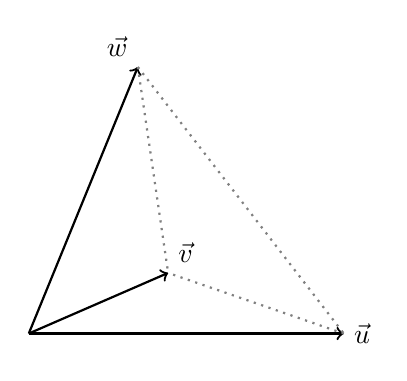
\begin{tikzpicture}
\coordinate (0) at (0,0,0);
\draw[thick, ->] (0)--(4,0,0) node[right](vecu){$\vec{u}$};
\draw[thick, ->] (0)--(1,0,-2) node[above right](vecv){$\vec{v}$};
\draw[thick, ->] (0)--(1,3,-1) node[above left](vecw){$\vec{w}$};
\draw[thick, gray, dotted] (4,0,0)--(1,0,-2);
\draw[thick, gray, dotted] (1,3,-1)--(1,0,-2);
\draw[thick, gray, dotted] (1,3,-1)--(4,0,0);
\end{tikzpicture}
\end{center}
\end{Exercise}

\begin{Exercise}
For $\vec{u} = (1,2,3)^T$, $\vec{v} = (2,1,5)^T$, $\vec{w} = (1,4,0)^T$, find
\begin{enumerate}[label=(\alph*)]
\item Area of the parallelogram formed by $\vec{u}$ and $\vec{v}$,
\item Volume of the parallelepiped formed by $\vec{u}$, $\vec{v}$ and $\vec{w}$,
\item Redo the above for $\vec{w} = (1,5,4)^T$, what does the result tell you?
\end{enumerate}
\end{Exercise}

\begin{Exercise}
Find the geometric interpretation of solutions of the following systems of linear equations.
\begin{enumerate}[label=(\alph*)]
\item \begin{align*}
\begin{cases}
x + 2y + 2z &= 3\\
3x - y + 3z &= 2\\
x - 2y - z &= -1
\end{cases}
\end{align*}
\item
\begin{align*}
\begin{cases}
2x - y - z &= 3\\
x + y + 2z &= -1\\
x + 4y + 7z &= -6
\end{cases}
\end{align*}
\end{enumerate}
\end{Exercise}

\begin{Exercise}
\begin{enumerate}[label=(\alph*)]
\item Find a parameterization for $x^2 + 3y^2 = 4$, by using sine and cosine, and considering related trigonometric identity,
\item Find the direct relationship for $x = 4t^2 + 3t + 5$, $y = 2t + 1$,
\item Describe the geometric shape for the curve $x = \cos{t}$, $y = \sin{t}$, $z = \frac{t}{\pi}$.
\end{enumerate}
where $-\infty < t < \infty$.
\end{Exercise}